 %% Copyright (C) 2006 Ahmer Ahmedani

\documentclass[MSc,twoside,openright]{Thesis}

\newif\ifdraft
% \drafttrue

%== Preamble ==================================================================

\usepackage[french]{babel}
\usepackage[T1]{fontenc}
\usepackage[utf8]{inputenc}

\usepackage{placeins}
\usepackage{tabularx}
\usepackage{multicol}
\usepackage{xcolor}    % Keyword highlighting in listing
\usepackage{listings}  % Typeset source code listings,
                       % Files in current direcotry
                       % ( listings.cfg listings.sty lstdoc.sty lstlang1.sty
                       % lstlang2.sty lstlang3.sty lstmisc.sty ) are listings
                       % version 1.4, should not be removed, 1.3 version cause
                       % problem in the left line of the frame (standalone use
                       % of 1.3 will not cause this problem, but in this
                       % project, it does)
\usepackage[bw]{mcode} % mcode listings

\usepackage{ifthen}    % For conditional commands
\usepackage{ifpdf}     % Provide \ifpdf conditional
\usepackage{xspace}    % Define commands that don't eat spaces
\usepackage{type1cm}
\usepackage{times}     % Use Times *deprecated*
%% listings.sty doesn't seem to pretty print code listings if the
%% `times' packages is not loaded. Why? Who knows. It will do it fine
%% in a simple document, just not in this one.
\usepackage{mathptmx}  % Use Times for roman family and math
% \usepackage{mathpazo}  % Palantino
% \usepackage{chancery}
% \usepackage{bookman}
% \usepackage{newcent}
% \usepackage{charter}
\usepackage[scaled]{helvet}    % Use Helvetica for sans serif family
%\usepackage{avant}     % Use Avant Garde for sans serif family
\usepackage{pifont}    % Symbol and Zapf Dingbats
%% TODO: investigate fourier package (Adobe Utopia fonts)

\usepackage{fancyhdr}  % Fancy page headers
\usepackage{verbatim}  % provide comment environments
\usepackage{fancyvrb}  % improved verbatim and verbatim* environments

%\usepackage{hyperref} % split urls
\usepackage{url}       % For nicely formatted URLs


%% Nicer formatting of figure captions:
\usepackage[format=hang,font={small,sf},labelfont=bf,labelsep=space]{caption}
%\usepackage[tight]{subfigure} % subfigures. replace with subfig?
\usepackage{subfig}
\usepackage{setspace}
\usepackage{longtable} % Make tables span multiple pages
\usepackage{multirow}  % Table cells that span multiple rows
\usepackage{dcolumn}   % Line up decimal sep in tabular columns
% \usepackage{warpcol}   % Alternate to dcolumn
\usepackage{color}     % Allows text and page background colors to be set
\usepackage{colortbl}  % Coloured tables
\usepackage[final]{graphicx}  % Better support for graphics
\usepackage{layout}    % produces a figure that describes the page layout
\usepackage{titlesec}  % to redefine typesetting of \paragraph
\usepackage{rotating}  % for rotated table headings
% Note: yap does not support rotating, so convert .dvi to .pdf and then
%    preview the .pdf file
% for algorithms
\usepackage[algo2e, algochapter, ruled, linesnumbered, lined]{algorithm2e}
%% Make sure that the bibliography is listed in the table of contents,
%% but that the table of contents itself is not.
% XXX: doesn't seem to work
%\usepackage[nottoc]{tocbibind}
\usepackage[none]{tocbibind}
%\usepackage{hyphenat} %enhanced hyphenation,
%\usepackage[htt]{hyphenat} %htt enables hyphenation of text typeset
% some better colours for hyperref links:
\definecolor{darkgreen}{rgb}{0.2,0.5,0.1}
\definecolor{darkblue} {rgb}{0.1,0.4,0.5}
\definecolor{maroon}   {rgb}{0.45,0.05,0.25}
\definecolor{red}      {rgb}{1,0,0}
\ifpdf
  %% TODO: can I use variables here for name, title, etc?
  \usepackage[
    pdftex,
    colorlinks=true,
    linkcolor=maroon,
    citecolor=darkgreen,
    pagecolor=maroon,
    urlcolor=darkblue,
    pdftitle={The MetaLexer Lexer Specification Language},
    pdfauthor={Andrew Casey},
    pdfsubject={The MetaLexer Lexer Specification Language},
    pdfkeywords={MetaLexer, Lexer, Scanner, Extensible, Modular}
  ]
  {hyperref} % hyper-text links, etc.
\else
  \usepackage[
    dvips,
    breaklinks=true,
    colorlinks=true,
    linkcolor=maroon,
    citecolor=darkgreen,
    pagecolor=maroon,
    urlcolor=darkblue,
  ]
  {hyperref}
\fi


% Use the ams math packages
\usepackage{amssymb,amsmath}
\usepackage{bnf}

% -- Customize Layout ---------------------------------------------------------

% custom page headers:

\lhead[]{\fancyplain{}{\nouppercase{\rightmark}}}
\rhead[\fancyplain{}{\nouppercase{\leftmark}}]{}
\addtolength{\headwidth}{10mm} % => extend line out into margin

%\fancyhead[EL]{THESIS DRAFT}
%\fancyhead[OR]{THESIS DRAFT}


\titleformat{\paragraph}[hang]{\normalfont\it}{}{0em}{}

% Make LaTeX relax a little wrt figure placement
\renewcommand{\topfraction}{0.85}
\renewcommand{\textfraction}{0.1}
\renewcommand{\floatpagefraction}{0.75} % Prevent half-empty pages

% Tell LaTeX to not "bottom justify" text. This prevents ugly
% spaces between paragraphs in columns when LaTeX stretches them.
\raggedbottom

% Set the depth for the table of contents to 2 for non-draft output
\ifdraft
\else
\setcounter{tocdepth}{2}
\fi

% Set the value of the margin of all algorithms.
% The default value is \leftskip plus \parindent
%  when the algorithm2e package is loaded.
\incmargin{\parindent} %increase one more \parindent to the default
% Set font of comment in algorithms
\newcommand{\algcommentfont}[1]{{\small \texttt{#1}}}
\SetCommentSty{algcommentfont}

%----------Matlab---------------------
\newcommand{\abc}{\textsl{abc}\xspace}
\newcommand{\amc}{\textsl{amc}\xspace}
\newcommand{\matlab}{{\sc Matlab}\xspace}
\newcommand{\smatlab}{{\sc Matlab}}
\newcommand{\smclab}{\textrm{\textsl{Mc}\textbf{\textsc{Lab}}}}
\newcommand{\mclab}{\smclab\xspace}
\newcommand{\mcirs}{\textrm{\textsl{Mc}\textbf{\textsc{ir}}}}
\newcommand{\smcir}{\mcirs}
\newcommand{\mcir}{\smcir\xspace}
\newcommand{\mcasts}{\textrm{\textsl{Mc}\textbf{\textsc{ast}}}}
\newcommand{\smcast}{\mcasts}
\newcommand{\mcast}{\smcast\xspace}
\newcommand{\smcjit}{\textrm{\textsl{Mc}\textbf{\textsc{jit}}}}
\newcommand{\mcjit}{\smcjit\xspace}
\newcommand{\java}{\textsc{Java}\xspace}
\newcommand{\sjava}{\textsc{Java}}
\newcommand{\fortran}{\textsc{Fortran}\xspace}
\newcommand{\mcbench}{{\sc McBench}\xspace}
\newcommand{\mcfor}{{\sc McFor}\xspace}
\newcommand{\mcsaf}{{\sc McSaf}\xspace}
\newcommand{\kw}[1]{\texttt{#1}}


\newcommand{\rednote}[1]{#1} %{\textcolor{red}{#1}}
\newcommand{\mynote}[1]{} %{\marginpar{\scriptsize{\rednote{#1}}}}

% MATLAB lang. def. for listings
\lstdefinelanguage{MATLAB}{
    sensitive=true, % Case sensitive identifiers
    morecomment=[l]{\%}, % Line-based comment character
    morestring=[b]', % String character
    morekeywords= {
		function,
		for,
		while,
		if,
		else,
		elseif,
		end,
		aspect,
		patterns,
		actions,
		methods,
		properties,
		class,
		classdef,
		script,
		loops,
		set,
		get,
		call,
		execution,
		mainexecution,
		loop,
		loopbody,
		loophead,
		within,
		before,
		after,
		around
	},
	commentstyle=\color[rgb]{.600,.600,.600}, % grey comments
}

% -- Input local commands and hyphenation rules -------------------------------
% -- Custom Environments ---
\definecolor{darkgrey} {rgb}{0.843,0.843,0.843}
\definecolor{lightgrey} {rgb}{0.979,0.979,0.979}
\lstset{
        language=[AspectJ]Java, %keyword highlighting seems annoying
        morekeywords={declare, parents},
        basicstyle=\ttfamily\footnotesize, % use fixed-width font
        keywordstyle=\bfseries\color[rgb]{.498,.000,.333}, % eclipse color, bold
        %keywordstyle=\bfseries, % bold keywords
        identifierstyle=,       % nothing happens
        %commentstyle=\color[rgb]{.247,.498,.372}, % eclipse color
        commentstyle=\color[rgb]{.753,.753,.753}, % grey comments
        stringstyle=\color[rgb]{.164,.000,1.00},  % eclipse color
        %stringstyle=\ttfamily,  % typewriter type for strings
        showstringspaces=false, % no special string spaces
	    tabsize=2,
        columns=fullflexible,   % Use flexible column format (for comments)
        frame=single, %
        framerule=0.6pt, %
        backgroundcolor=\color{white}, %
        rulecolor=\color{darkgrey}, %
        captionpos=b, %
	    numbers=left, 
	    numberstyle=\scriptsize\color[rgb]{.501,.501,.501},
	    stepnumber=1,
	    breaklines=true,
	    breakatwhitespace=true
}

\newcommand{\code}[1]{{\small \texttt{#1}}}
\newcommand{\codekeyword}[1]{\textbf{\code{#1}}}

% MetaLexer

\newcommand{\mlkw}[1]{\codekeyword{#1}\xspace}
\newcommand{\ml}[1]{\textit{#1}}
\newcommand{\jflexkw}[1]{\codekeyword{#1}\xspace}
\newcommand{\jflex}[1]{\textit{#1}}
%\newcommand{\java}[1]{\textit{#1}}
\newcommand{\weburl}[1]{\textit{#1}}
\newcommand{\file}[1]{\textit{#1}}
\newcommand{\target}[1]{\textit{#1}}
\newcommand{\property}[1]{\textit{#1}}
\newcommand{\cli}[1]{\textit{#1}}
\newcommand{\chapref}[1]{\textit{Chapter \ref{#1}}}
\newcommand{\appendixref}[1]{\textit{Appendix \ref{#1}}}
\newcommand{\sectionref}[1]{\textit{Section \ref{#1}}}
\newcommand{\figref}[1]{\textit{Figure \ref{#1}}}
\newcommand{\tableref}[1]{\textit{Table \ref{#1}}}
\newcommand{\lstref}[1]{\textit{Listing \ref{#1}}}
\newcommand{\lstrefTwo}[2]{\textit{Listings \ref{#1} \& \ref{#2}}}
\newcommand{\lstrefN}[2]{\textit{Listings \ref{#1} - \ref{#2}}}

\newcommand{\secref}[1]{Sec.~\ref{#1}}
\newcommand{\figureref}[1]{Figure~\ref{#1}}
\newcommand{\equationref}[1]{Equation~\ref{#1}}
\newcommand{\eqnref}[1]{(\ref{#1})}
\newcommand{\RC}{reference-counting-based }



\newcommand{\patANY}{\mlkw{<<ANY>>}}
\newcommand{\patEOF}{\mlkw{<<EOF>>}}
\newcommand{\mpatANY}{\mlkw{<ANY>}}
\newcommand{\mpatBOF}{\mlkw{<BOF>}}

\newcommand{\red}[1]{\textcolor{red}{#1}}
\newcommand{\note}[1]{\textcolor{red}{\textbf{#1}}}
\newcommand{\variation}[2]{\textbf{\textcolor{green}{#1} \red{or} \textcolor{blue}{#2}}}

%\newcommand{\mcode}[1]{\lstinline[language=MATLAB]|#1|}
\newcommand{\jcode}[1]{\lstinline[language=Java]|#1|}
\newcommand{\pcode}[1]{\lstinline[language=pseudo]|#1|}


\newcommand{\into}{ 
   \end{minipage}
   \parbox{1cm}{\LARGE\centering $\mathbf{\Rightarrow}$}
   \begin{minipage}{5cm}
 }
\newenvironment{transform}
{
  \begin{center}
    \begin{minipage}{5cm}
}
{
  \end{minipage}
\end{center}
}
\lstnewenvironment{mtrans}
{
\lstset{language=matlab,numbers=none,frame=single}
}
{}

%%% Local Variables:
%%% mode: LaTeX
%%% TeX-master: "thesis"
%%% End: 


% Make matlab the default language
\lstset{
  language=MATLAB,
  mathescape=true
}

%== Title Information =========================================================

%--------------------- 70 character title limit -----------------------
\title{TITLE TO BE DETERMINED}

\author{Ismail Badawi}

\Department{School of Computer Science}
\Institution{McGill University}
\Location{Montr\'eal}

\SubmitDate{Submission date to be determined}

\CopyrightMessage{Copyright \copyright\ 2014 Ismail Badawi}

%== Document ==================================================================

\begin{document}

\pagestyle{empty}

\maketitle
\cleardoublepage

\preface % -- Front Matter ----------------------------------------------------

\begin{Abstract}

\matlab is a dynamic scientific language used by scientists, engineers and
students worldwide.  Although \matlab is very suitable for rapid prototyping
and development,  \matlab users
often want to convert their final \matlab programs to a static language such as {\sc
FORTRAN}, to integrate them into already existing programs of that language,
to leverage the performance of powerful static compilers, or to 
ease the distribution of executables.

This thesis presents an extensible object-oriented toolkit to help
facilitate the generation of static programs from dynamic \matlab
programs.  Our open source toolkit, called the \matlab Tamer, targets
a large subset of \matlab. Given information about the entry point of
the program, the \matlab Tamer builds a complete callgraph, transforms
every function into a reduced intermediate representation, and
provides typing information to aid the generation of static code.

In order to provide this functionality, we need to handle a large
number of \matlab builtin functions. Part of the Tamer framework is
the builtin framework, an extensible toolkit which provides a
principled approach to handle a large number of builtin functions.  To
build the callgraph, we provide an interprocedural analysis framework,
which can be used to implement full-program analyses.  Using this
interprocedural framework, we have developed value analysis, an extensible
interprocedural analysis to estimate \matlab types, which helps
discover the call edges needed to build the call graph.

In order to make the static analyses even possible, we disallow a
small number of \matlab constructs and features, but attempt to
support as large a subset of \matlab as possible.  Thus, by both
slightly restricting \matlab, and by providing a framework with
powerful analyses and simplifying transformations, we can
``Tame \matlab''.





\end{Abstract}

\begin{Resume}
{\sc Matlab}\textsuperscript{\textregistered} est un langage de programmation
dynamique populaire chez les scientifiques. L'utilisateur typique de \matlab
n'est pas un programmeur professionel; \matlab est
principalement utilis\'{e} par des scientifiques, des ing\'{e}nieurs et des
\'{e}tudiants, et doit sa popularit\'{e} en grande mesure \`{a} sa syntaxe de
haut niveau et \`{a} son \'{e}ventail de librairies pour toutes sortes de
domaines dans les sciences. Le manque d'\'{e}xperience des programmeurs
\matlab, combin\'{e} \`{a} ses s\'{e}mantiques mal sp\'{e}cifi\'{e}es et
souvent contraires \`{a} l'intuition, m\`{e}ne \`{a} du code \matlab qui est
difficile \`{a} comprendre et maintenir.

Dans cette th\`{e}se, nous pr\'{e}sentons McIDE, un environnement de
d\'{e}veloppement int\'{e}gr\'{e} pour \matlab. McIDE fournit des outils visant
\`{a} aider les programmeurs \matlab \`{a} \'{e}crire de meilleurs programmes,
incluant des remaniements automatiques et des fonctions de navigation de code,
par exemple permettant de sauter \`{a} la d\'{e}finition d'une fonction. McIDE
a aussi des avis tr\`{e}s arr\^{e}t\'{e}s sur le code \matlab, et tente de
reconna\^{i}tre des motifs probl\'{e}matiques courants et soit d'avertir le
programmeur ou de les \'{e}liminer automatiquement.

McIDE est compos\'{e} de plusieurs composants plus-ou-mains autonomes,
connect\'{e}s par une interface graphique assez mince. Certains de ces
composants existaient d\'{e}j\`{a}, tel qu'un parseur de \matlab fournit par le
projet \mclab, tandis que d'autres forment les contributions de cette
th\`{e}se, comme un m\'{e}chanisme pour d\'{e}couvrir le graphe d'appels
dynamiques de code \matlab, et un outil pour transformer du code de mani\`{e}re
\`{a} pr\'{e}server sa mise en page.

\`{A} travers la mise en oeuvre de McIDE, un th\`{e}me courant est la
d\'{e}pendance sur de l'information r\'{e}colt\'{e}e en cours
d'\'{e}x\'{e}cution, puisque l'information statique est souvant insuffisante si
nous souhaitons supporter le d\'{e}veloppement de code \matlab arbitraires,
incluant ses fonctions plus dynamiques.

\end{Resume}

\chapter*{Acknowledgements}
I'd like to thank my advisor Laurie Hendren, who displayed a lot of patience,
even when it wasn't clear whether I was making forward progress.

I'd like to thank the Sable lab members and alumni I've interacted with during
the time that I've spent here -- among them Anton Dubrau, Matthieu Dubet, Xu Li,
Vineet Kumar, Rahul Garg, Sameer Jagdale, Faiz Khan, Sujay Kathrotia, Vincent
Foley-Bourgon and Erick Lavoie.

I'd particularly like to thank my friends Jerina Harizaj and Lei Lopez, who
were positive forces in my life during periods where I felt very frustrated and
dispirited.

Finally, I'd like to thank my parents, my brother and my sister for their
lifelong support and encouragement.



\renewcommand{\contentsname}{Table of Contents}%
\addto\captionsenglish{%
  \renewcommand{\contentsname}%
    {Table of Contents}%
}
\addto\captionsenglish{%
  \renewcommand{\lstlistlistingname}%
    {List of Listings}%
}

\tableofcontents
\listoffigures
\listoftables
% Make the 'list of listings' page follow the conventions for the title
\renewcommand{\lstlistlistingname}{List of Listings}
%This line results in a duplicate entry in the .out file
%\renewcommand{\lstlistoflistings}{\begingroup
%  \tocfile{\lstlistlistingname}{lol}
%\endgroup}
%\lstlistoflistings
%\listoflistings
%\listofalgorithmes
\cleardoublepage

\maintext % -- Main Body ------------------------------------------------------

\pagestyle{fancyplain}

\chapter{Introduction} \label{chap:Introduction}
\matlab is a popular numeric programming language, used by millions of
scientists, engineers and students worldwide\cite{MatlabGrowth}.  \matlab
programmers appreciate the high-level matrix operators,  the fact that
variables and types do not need to be declared, the large number of library and
builtin functions available, and the interactive style of program development
available through the IDE and the interpreter-style read-eval-print loop.
However, even though \matlab programmers appreciate all of the features that
enable rapid prototyping,  they often have other ultimate goals.  Frequently
their computations are quite computationally intensive and they really want an
efficient implementation.  Programmers also often want to integrate their
\matlab program into existing static systems.  As just one example, one of our
users wanted to generate {\sc FORTRAN} code that can be plugged into a weather
simulation environment.    

This thesis addresses the problem of how to provide the bridge between
the dynamic realities of \matlab and the ultimate goal of wanting
efficient and static programs in languages like {\sc FORTRAN}.  It is
not realistic to support all the \matlab features, but our goal is to
define and provide support for a very large subset of \matlab which
includes dynamic typing, support of the \matlab function lookup
semantics, variable numbers of input and output arguments, support for
a variety of \matlab data types including arrays, cell arrays and
structs, and support for function handles and lambda expressions.

Providing this bridge presents two main challenges.  The first is that \matlab
is actually quite a complex language which has evolved over many years and
which has non-standard type rules and function lookup semantics.  The second
major challenge is properly dealing with the large number of builtin and
library functions,  which have also been developed over time and which
sometimes have unexpected or irregular behavior. 

\begin{figure}[htbp]
\begin{center}
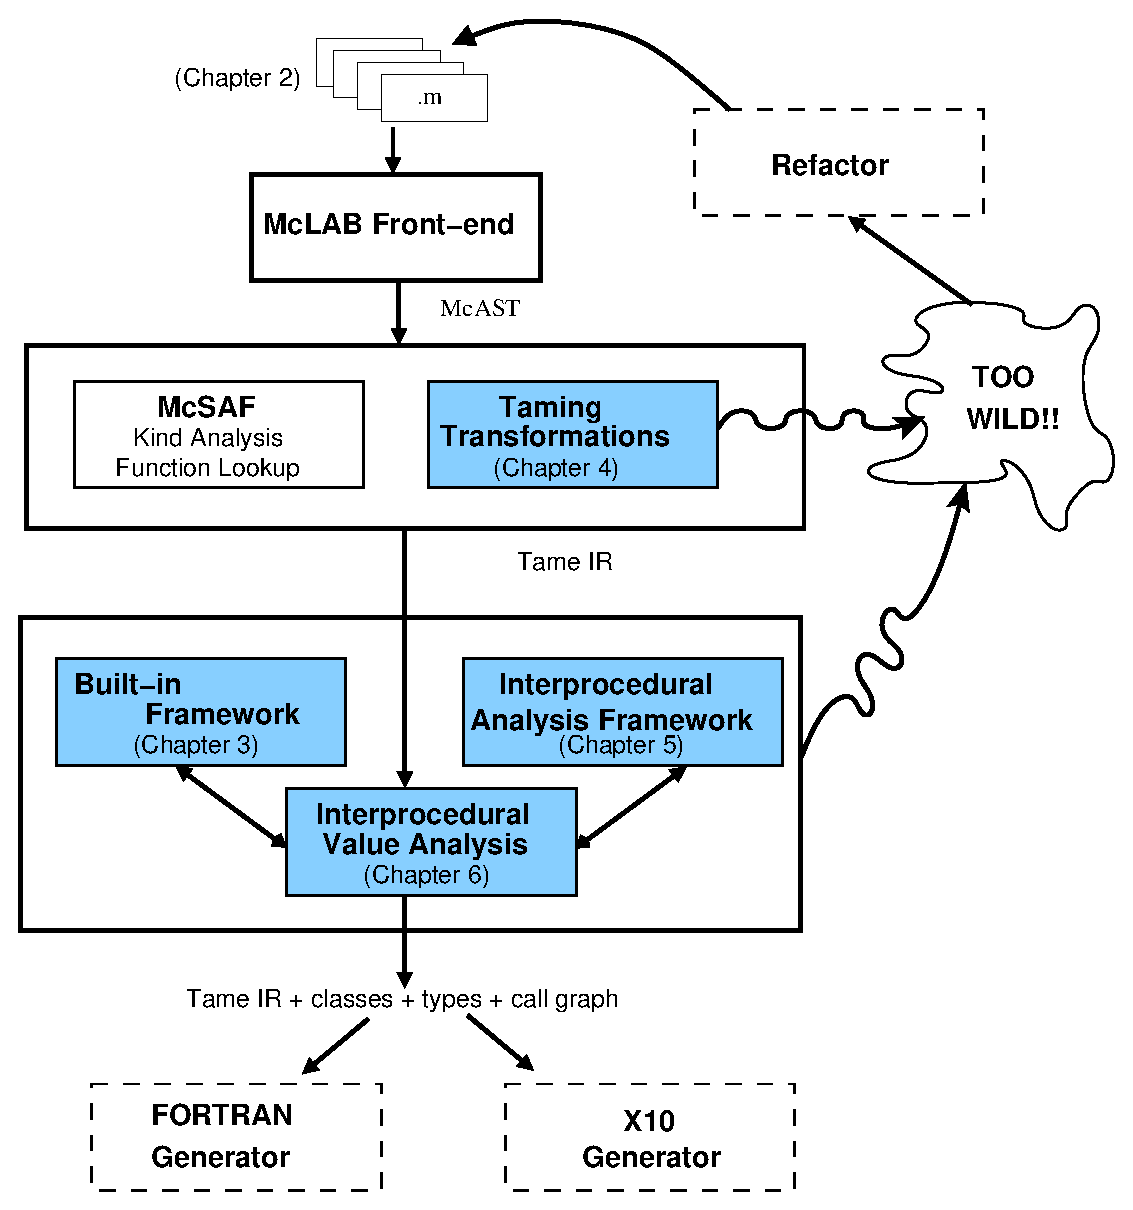
\includegraphics[width=3.5in]{Figures/overview.eps}
\caption[Overview of the \matlab Tamer]{Overview
of our \matlab Tamer.  The shaded boxes indicate the components
presented in this thesis.  The other solid boxes correspond to
existing \mclab tools we use, and the dashed boxes correspond to
ongoing projects which are using the results of this
thesis.}\label{Fig:Overview}
\end{center}
\end{figure}

Our solution is an open-source extensible objected-oriented framework,
implemented in Java, as presented in \figref{Fig:Overview}.   The overall
goal of the system is to take \matlab programs as input and produce output
which is suitable for static compilation, a process that we call
\textit{Taming} \matlab.   Given a \texttt{.m} file as input, which is the
entry point, the \matlab Tamer produces as output: (1) a Tame
IR \rednote{(intermediate representation)} for all functions (both user
and library) which are reachable from the entry point, (2) a complete
call graph, and (3) an estimation of classes/types for all variables.

There are some features in \matlab that are simply too wild to handle, and so
our system will reject programs using those features, and the user will need to
refactor their program to eliminate that feature.   Thus, another important
goal in our work is to define as large as possible subset of \matlab that can
be tamed without user intervention. 

\section{Contributions}

The main contributions of this thesis are as follows.

\begin{itemize}
\item We present an overall design and implementation for the \matlab Tamer,
an extensible object-oriented framework
which provides the bridge between the dynamic \matlab language and a static back-end
compiler. 

\item We describe the key features of \matlab necessary for compiler developers
and for tool writers to understand \matlab and the analyses in this thesis.  We hope
that by carefully explaining these ideas, we can enable other researchers
to also work on static tools for \matlab.  Our discussion of \matlab features
also motivates our choice of the subset of \matlab that we aim to tame. 

\item We provide a principled approach to understanding, grouping, and
analyzing the large number of \matlab builtin functions.

\item We developed extensions to the \mcsaf\cite{JesseThesis} framework to support a lower-level
and more specialized Tame IR, suitable for back-end static code generation.

\item We present an interprocedural flow analysis framework that allows
 extending intraprocedural analysis written for the \mcsaf framework to
 analyze whole programs.
 
\item We present an interprocedural flow analysis framework that computes both
abstract values and the complete call graph.  This flow analysis
provides an object-oriented approach which allows for extension and
refinement of the abstract value representations.

\end{itemize}


\section{Thesis Outline}
This thesis is divided into \ref{chap:Conclusions} chapters, including this one, which are structured as follows.

\chapref{chap:MATLAB} introduces key \matlab features,
showing some of the challenges of static compilation.
\chapref{chap:Builtin} describes our
approach to dealing with \matlab builtin functions, starting with some
examination of which builtin functions are relevant, and how they
behave.
\chapref{chap:TameIR} presents the Tame IR and
transformations, including how these were integrated with the existing
analysis framework.
\chapref{chap:inter} describes our interprocedural analysis framework.
\chapref{chap:ValueAnalysis} explains our 
extensible and modular interprocedural value analysis and how it
constructs complete callgraphs. We also show some results of running
this analysis on a set of benchmarks.
\chapref{chap:Related} provides an overview of related work and
\chapref{chap:Conclusions} concludes.


\chapter{Layout-preserving Refactorings} \label{chap:Layout}
A refactoring is a code transformation that changes the structure of the code
while preserving its semantics, and can often naturally be thought of as a
transformation over the structure of an abstract syntax tree. However, from
the perspective of a programmer using a refactoring tool, a refactoring is
ultimately a textual transformation. It is important to reconcile these two
conceptions of refactorings; purely working in terms of ASTs, while
technically correct from a semantics perspective, is apt to lose a lot
of information about the textual layout of the code, while purely working
in terms of text is apt to make implementations of individual refactorings
very brittle, hard to reason about, and hard to maintain.

In this chapter, we present our approach to making refactorings layout
preserving.  We allow refactorings to be implemented in terms of a minimal tree
transformation API, which hides the mechanics of layout preservation. As
refactoring writers specify tree-level edits, minimal text-level edits are
transparently computed from them. This simplifies the implementations of
individual refactorings, allowing them to remain oblivious to the program text,
while making them directly usable by end-users.

\section{Motivation}

Once all the issues surrounding semantics-preservation -- running required
analyses, checking required preconditions, and so on -- are sorted out,
then from an implementation perspective, a refactoring is most
naturally thought of as a transformation on abstract syntax trees. For
instance, a refactoring like "extract method" can be boiled down to steps like
"move this statement from this function to that one", "synthesize a new
function call", and "replace that statement with this one", and so
on. Given this, a natural structure for a refactoring tool consists of parsing
code, then performing transformations on its AST, and then pretty printing the
transformed AST to retrieve source code to present to the programmer. Many
refactoring tools -- particularly ones developed for research purposes, where
practicality is often a non-goal -- operate this way.

The problem with such approaches is that by construction the AST does not
contain enough information to accurately reconstruct the input source code.
Typically among the casualties are whitespace, comments, and syntactic sugar.

\figref{Fig:LostLayout} shows a \matlab program and the result of parsing and
then pretty-printing it using the \mclab toolkit. The two programs are
behaviorally equivalent, but contain many syntactic differences. The comment
associated with the \code{cube} function has moved below the header. The
four-space indentation has been changed to two-space indentation. Each binary
expression has been wrapped in parentheses.  The output parameters have been
wrapped in square brackets.  The nested function \code{square} has been moved
-- in \matlab, nested functions have the same scope irrespective of where they
are declared; as a simplification, the Natlab translation moves nested
functions to the bottom of their enclosing function.

\begin{figure}
\begin{minipage}{0.5\linewidth}
\begin{lstlisting}[numbers=none]
% cube takes a number x and returns its cube.
function y = cube(x)
    % This is a nested function that computes the square of a value.
    function v = square(u)
        v = u * u;
    end
    y = x * square(x);
end
\end{lstlisting}
\end{minipage}
\hfill \hspace{.3cm} \hfill
\begin{minipage}{0.5\linewidth}
\begin{lstlisting}[numbers=none]
function [y] = cube(x)
  % cube takes a number x and returns its cube.
  % This is a nested function that computes the square of a value.
  y = (x * square(x));
  function [v] = square(u)
    v = (u * u);
  end
end
\end{lstlisting}
\end{minipage}
\caption{An example of the lossy parsing and unparsing roundtrip.}
\label{Fig:LostLayout}
\end{figure}

Users of an automated refactoring tool are unlikely to be accepting of such
invasive changes to a program's text. As such, it is important for the tool to
be aware of the layout of the program when performing refactorings. For a given
AST transformation, it should endeavor to perform the minimal textual changes
needed to reflect the transformation in the program text. In particular,
unaffected portions of the program should not undergo any textual changes.

Despite this, it is still convenient to express refactorings as tree
transformations. Refactorings would be much harder to implement and maintain if
they had to be expressed as textual transformations, or as a mixture of tree
and text transformations that had to be kept in sync.

Our goal is to be able to implement refactorings purely as tree
transformations, and to have minimal textual changes automatically computed
from them. In order to accomplish this, we introduce a simple transformation
API, which exposes a small set of tree manipulation operations. Instead of
directly manipulating AST nodes, refactorings are implemented in terms of this
API. Behind the scenes, the implementation of the API includes logic that keeps
track the input program text in addition to the AST, and keeps the two in sync.

\section{Synchronizing ASTs and token streams}

At a high level, our approach to layout preservation works as follows. Given a
\matlab source file, we start by tokenizing the source code using a \matlab
lexer, yielding a stream of tokens. Alongside the token stream, we use a
\matlab parser to parse the same source file, yielding an abstract syntax tree.
Our aim is to allow refactoring writers to specify edits to the abstract syntax
tree, and to have those edits be transparently reflected in the token stream.
In the end, when the time comes to present the transformed source back to the
user, we can simply concatenate all the tokens instead of pretty printing the
AST.

In order for this to work, there are two "primitives" that we rely on. First,
we need to be able to identify, for a particular AST node (which may be a node
from the original program, or a copy of a node, or a brand new synthesized
node), the portion of the token stream corresponding to that node. Second, we
need to be able to make local modifications to just that portion of the stream,
without compromising our ability to later look up nodes in the modified stream.

To bridge the gap between the token stream and the AST, we use position
information. Each token consists of a fragment of text together with a line and
column position where it occurs in the source code. Each AST node, assuming it
was produced by the parsing process and not manually synthesized after the
fact, also contains position information. As an initial link between the source
text and the AST, we can simply create a table that maps line and column
positions to the corresponding token in the stream. When we need to retrieve
the portion of the token stream for a given node, we can simply look up the
token corresponding to its start position, look up the node token corresponding
to its end position, and take all the tokens in between.

One potential complication here is that the mapping could become stale as the
token stream is modified. For instance, if we were to simply keep an array of
tokens and map positions to indices into the array, then as the stream is
edited and tokens are shifted around, indices would no longer point to the same
token. In some cases we may be able to update the mapping as we edit the
stream, but that approach quickly becomes brittle and hard to reason about.

In order to avoid this complication, and also to satisfy our requirement of
supporting local edits to the token stream, it is necessary to carefully
consider the data structure we will use to represent the token stream. A
natural choice is a doubly linked list. The values in our table can be
references to individual nodes in the list, which will remain valid even as
their positions within the list change. Also, since each node contains a
reference to its predecessor and successor within the list, we can cheaply
support edits like removing a sequence of tokens, or inserting a sequence of
tokens before or after a particular token.

A common operation when implementing refactorings is to a copy an AST
node. Since this approach associates mutable state (a portion of the token
stream) with each node, it's not enough to simply copy the node; the
corresponding token stream fragment should be also be copied, and the copy
associated with the newly copied node. We will see later that `copy(ASTNode)`
is an operation exposed by the transformation API.

That suffices for correlating the token stream with the AST of the original
source text, but we need to be able to maintain this mapping as the token
stream is edited, code is moved around or copied, and new code is synthesized.

\section{Dealing with freshly synthesized code}

It is common for refactorings to insert new code into the program which wasn't
present in the original source text. For example, in the case of extract
method, a new function call is synthesized to replace the extracted statements,
a new function is synthesized to hold them, and that new function might also
contain some synthetic statements like global variable declarations to ensure
semantics are preserved. These pose a problem since there is no original text
to tokenize in this case.

The natural intuition is to somehow leverage the output of the pretty printer
to recover some text that we may integrate into the token stream. If we simply
pretty print the new AST, we get a program fragment as a string that we can
then feed to the lexer. However, since these synthetic AST nodes don't have
position information, we can't easily associate nodes with their portion of the
token stream. We can associate the top-level tree with the entire fragment, but
subtrees pose a problem.

One way to deal with this would be to pretty print the new AST to recover the
program text, then parse the text again to get back an AST that has position
information, and then proceed as before. This is viable, but it implies that
all new nodes would have to be synthesized through the tree transformation API
-- nodes that are synthesized by the caller directly couldn't be used, since
they wouldn't have the necessary position information.

In the interest of keeping the API surface small, we instead implement a
tokenizing pretty printer, which is a version of the pretty printer that emits
sequences of tokens instead of entire strings. This can implemented as a
straightforward recursive traversal of the AST; for each node, we synthesize a
sequence of tokens, and at the same time associate that sequence with the node
for later use.

Given this, we can now look up the relevant portion of a token stream for a node
by first checking if it has a fragment explicitly associated with it by the
pretty printer, and otherwise using its position information to look it up in
our original mapping.

\section{The transformation API}
All AST manipulation can be boiled down to a series of node deletions and insertions.
A replace operation is also convenient, and as mentioned previously a copy operation
is required by our approach to layout preservation. Finally, an operation to recover
the transformed source code is also needed. \figref{Fig:TransformerAPI} shows how
these operations are encoded as a Java interface.

\begin{figure}
\begin{lstlisting}[numbers=none, language=Java]
public interface Transformer {
  void replace(ASTNode<?> node, ASTNode<?> newNode);
  void remove(ASTNode<?> node);
  void insert(ASTNode<?> node, ASTNode<?> newNode, int i);
  <T extends ASTNode<?>> T copy(T node);
  String reconstructText();
}
\end{lstlisting}
\caption{The Transformer API, encoded as a Java interface}
\label{Fig:TransformerAPI}
\end{figure}

\section{Case studies: inline variable, extract function}

The Inline Variable refactoring is relatively simple; it takes an assignment
statement as input, and replaces each use of the assigned variable with the
expression on the right hand side before removing the assignment.
\figref{Fig:InlineVariable} shows how the mechanics of the transformation are
implemented against the transformation API (skipping over the portions of the
code dealing with the correctness of the transformation).

\begin{figure}
\begin{lstlisting}[numbers=none, language=Java]
public class InlineVariable extends Refactoring {
  private AssignStmt definition;

  // constructors, correctness checks, ...

  public void apply() {
    Transformer transformer = context.getTransformer(definition);
    UseDefDefUseChain udduChain = definition.getMatlabProgram().analyze().getUseDefDefUseChain();
    for (Name name : udduChain.getUses(definition)) {
      transformer.replace(name.getParent(), transformer.copy(definition.getRHS()));
    }
    transformer.remove(definition);
  }
}
\end{lstlisting}
\caption{The implementation of the Inline Variable refactoring using the transformer API}
\label{Fig:InlineVariable}
\end{figure}

The Extract Function refactoring slightly more involved.
\figref{Fig:ExtractFunction} shows how the mechanics of the transformations are
implemented against the transformation API. Even though the refactoring moves
AST nodes around, copies nodes, and mixes in synthetic code with the original text,
the code is completely oblivious to text, instead leaning on the {\tt Transformer}
to do the heavy lifting.

\begin{figure}
\begin{lstlisting}[numbers=none, language=Java]
public class ExtractFunction extends Refactoring {
  private StatementRange extractionRange;
  private Function enclosingFunction;
  private String extractedFunctionName;

  // constructors, correctness checks, ...

  // Synthesizes a call to the extracted function. Since there is no
  // code to preserve, it doesn't use the transformation API.
  private Stmt makeCallToExtractedFunction() { /* ... */ }
  // Determines the extracted function's input parameters
  private List<String> inputVars() { /* ... */ }
  // Determines the extracted function's output parameters
  private List<String> outputVars() { /* ... */ }
  // Determines the global variables used by the extracted function
  private List<String> globalVars() { /* ... */ }

  public void apply() {
    Transformer transformer = context.getTransformer(enclosingFunction);
    Function extracted = new Function(extractedFunctionName);
    for (Stmt stmt : extractionRange) {
      transformer.insert(extracted.getStmts(), transformer.copy(stmt), extracted.getNumStmt());
    }

    extracted.addInputParams(inputVars());
    extracted.addOutputParams(outputVars());
    for (String var : globalVars()) {
      transformer.insert(extracted.getStmts(), new GlobalStmt(var), 0);
    }

    List<Function> functionList = ((FunctionList) enclosingFunction.getParent()).getFunctions();
    transformer.insert(functionList, extracted, functionList.getIndexOfChild(enclosingFunction) + 1);
    for (int i = 0; i < extractionRange.size(); ++i) {
      transformer.remove(extractionRange.getStartStatement());
    }
    transformer.insert(extractionRange.getEnclosingStatementList(),
      makeCallToExtractedFunction(), extractionRange.getStartIndex());
  }
}
\end{lstlisting}
\caption{The implementation of the Extract Function refactoring using the transformer API}
\label{Fig:ExtractFunction}
\end{figure}

\section{Related work}

The work that most closely resembles ours is HaRe, a refactoring tool for
Haskell.  It uses a similar approach of synchronizing an AST with a token
stream in order to pretty print refactored programs.

Waddington and Yao [LDTA '05] tackled the same problem, which termed "the
problem of style disruption", with Proteus, their refactoring tool for C and
C++. Their approach to use a specialized AST called a "Literal-Layout AST
(LL-AST)", where literals token and whitespace nodes are interspersed alongside
the regular nodes.

* RefactorErl * That Scala refactoring guy


The Eclipse JDT contains infrastructure for modifying code at two levels -- a
lower-level API for describing text manipulation primitives, and a higher-level
AST rewriting API, which accepts descriptions of changes to AST nodes and uses
the text manipulation API to try and perform the textual changes required to
represent the AST changes. The approach is similar to ours in spirit; one big
difference is that since that our approach is implemented largely a standalone
tool, we rely solely on lexing and parsing as primitives, while Eclipse's
implementation benefits from more sophisticated integration with a scriptable
text editor.


\chapter{Related Work} \label{chap:Related}
There are several categories of related work.  First, we have the
immediate work upon which we are building.  The \mclab project already
provided the front-end and the \mcsaf\cite{JesseThesis} analysis
framework, which provided an important basis for the Tamer.  
Then there is \mcfor, a previous attempt to build a static
compiler targeting {\sc FORTRAN95}, that is part of the \mclab project.
There are also other compilers for \matlab, both static ones and
dynamic ones.
\
There is also related work on statically analyzing and compiling
other dynamic languages, with some similar problems we have faced,
and some similar approaches. Some of this work is presented
in section \secref{sec:otherStatic}.

\section{\mcfor}

We learned a lot from \mclab's previous \mcfor project\cite{McForThesis}
which was a first prototype \matlab to {\sc FORTRAN95}
compiler.  \mcfor supported a smaller subset of the language, and
simply ignored unsupported features - leading to possibly undefined
behavior. \mcfor did also not have a comprehensive approach to the
builtin functions, did not support the \matlab function lookup semantics, and
had a much more ad hoc approach to the analyses.  However, it really
showed that conversion of \matlab to {\sc FORTRAN95} was possible, and
that {\sc FORTRAN95} is an excellent target language.
In particular it showed that the numerical and matrix features
of {\sc FORTRAN95} are a good match for compiled \matlab, and that
the static nature of the language, together with powerful
{\sc FORTRAN95} compilers provide the potential for high performance.

We have developed the Tamer with targeting {\sc FORTRAN95} in mind. In
order to provide some extra flexibility for other potential backends
we have restricted \matlab less than may be necessary for a \matlab to
{\sc FORTRAN} compiler, i.e. it may have to restrict the \matlab
language further. For example, {\sc FORTRAN95} has very limited
polymorphism support, meaning that any polymorphic code can not be
easily \rednote{translated} to compact and readable FORTRAN. \mcfor does observe
these limitations, but does have an interesting way to deal with one
polymorphic case: If an if-statement results in incompatible types for
a variable along both branches, the code following that if-statement
gets copied into both branches, so that there won't be a confluence of
incompatible types.  For example,
\vspace{-.5cm}
\begin{lstlisting}
if (...)
  x = 3
else
  x = 'Hi'
end
foo(x)
\end{lstlisting}
may be converted to
\vspace{-.5cm}
\begin{lstlisting}
if (...)
  x = 3
  foo(x)
else
  x = 'Hi'
  foo(x)
end
\end{lstlisting}
This transformation is not possible in general for confluence points around
loop statements, and does also not work if values with ambiguous types
are returned from a function.

Despite being a full compiler with many interesting ideas, \mcfor is a
prototype, with limited feature set and limited extensibility. For
this thesis we have gone back to the basics and defined a much larger
subset of \matlab, taken a more structured and extensible approach to
building a general toolkit, tackled the problem of a principled
approach to the builtins, and defined the interprocedural analyses in
a more rigorous and extensible fashion.  The next generation of \mcfor
can now be built upon these new foundations.

\section{Other Static \matlab compilers}

Although we were not able to find publicly available versions, there
have been several excellent previous research projects on static
compilation of \matlab which focused particularly on the array-based
subset of \matlab and developed advanced static analyses for
determining shapes and sizes of arrays.  For example,
FALCON \cite{falcon} is a \matlab to {\sc FORTRAN90} translator with
sophisticated type inference algorithms.  Our Tamer is targeting a
larger and more modern set of \matlab that includes other types of
data structures such as cell arrays and structs, function handles and
lambda expressions, and which obeys the modern semantics of \matlab7.
We should note that FALCON handled interprocedural issues by fully
in-lining all of the the code.  MaJIC\cite{MaJIC}, a MATLAB
Just-In-Time compiler, is patterned after FALCON.  It uses similar
type inference techniques to FALCON, but are simplified to fit the JIT
context.  MAGICA \cite{Joisha03,MAGICA} is a type inference engine
developed by Joisha and Banerjee of Northwestern University, and is
written in Mathematica and is designed as an add-on module used by
MAT2C compiler \cite{MAT2C}.  We hope to learn from the advanced type
inference approaches in these projects and to implement similar
approximations using our interprocedural value analysis.

There are also commercial compilers, which are not publicly available, and for
which there are no research articles.   One such product is the \textit{MATLABCoder} 
recently released by MathWorks\cite{MATLABCoder}.   This product
produces C code for a subset of \matlab.  According to our preliminary tests,
this product does not appear to support cell arrays except in very
specific circumstances, nor does it support a general form of lambda
expressions, and was therefore unable to handle quite a few of our benchmarks.  
However, the key differences with our work is that we are
designing and providing an extensible and open source toolkit for compiler and
tool researchers.   This is clearly not the main goal of proprietary compilers.

\section{Other \matlab-like systems}

There are other projects providing open source implementations of \matlab-like
languages, such as Octave\cite{Octave} and Scilab\cite{Scilab}.   Although
these add valuable contributions to the open source community,  
their focus is on providing interpreters and open library support and they have
not tackled the problems of static compilation.   Thus, we believe that our
contributions are complementary. In particular Octave may present opportunities
to improve the usefulness of our static compiler framework without requiring
an actual \matlab installation.
 Octave, being an interpreter system, may not provide very high
performance, but it does include a large library similar to \matlab's
library. Enabling our framework to support Octave's specific \matlab flavor
may help bring together Octave's completeness with the potential performance
gains of a static compilation framework.


\section{Static Approaches to other Dynamic Languages}
\label{sec:otherStatic}

Other dynamic languages have had very successful efforts in defining
static subsets in order to provide static analysis.

\subsection{Python}

Reduced Python (RPython)\cite{RPython} provided inspiration for our
approach at dealing with a dynamic language in a static way. Rather
than attempting to support dynamic features that are not amenable to
static compilation, for example by providing interpreter-like features
as a fallback, RPython restricts (``reduces'') the set of allowable features such
that programs are statically typable. At the same time, it attempts to
stay as expressive as possible.

RPython was originally developed for PyPy, a Python interpreter written \rednote{in} Python,
but has evolved into be a general purpose language.
It was not developed to compile programs completely statically,
but rather with the goal to speed up execution times in 
virtual machines like VM or CLI, which are themselves developed
for static languages (Java and C\#, respectively).

%boot strapping phase?

Besides disallowing dynamic features, RPython disallows a basic feature
of many dynamic programing languages: at a confluence point,
a variable may not be defined with two incompatible types. This
notion that a variable should have one specific type at every programming
point is something that we expect for static backends of our framework
as well, in particular for FORTRAN, even if the Tamer Framework itself
actually supports union types. Both RPython, as well as our own research
have indicated that this restriction is not a serious limitation in practice.

RPython restricts Python's container types. In particular, it forces
that dictionaries (hash-tables) and arrays are homogeneous, i.e. all
elements have the same type. Tuples are allowed to be inhomogeneous.
For the Tamer, we represent the two builtin container types (structs,
cells) in both possible ways: as a tuple or as a collection, which correspond to
inhomogeneous and homogeneous representations, respectively.

RPython does not directly support generic functions, i.e. if a function
is used multiple times with incompatible arguments, the program
gets rejected. The Tamer uses a context-sensitive interprocedural
analysis that creates copies of functions when they are called
with incompatible arguments.


\subsection{Ruby}
DiamondbackRuby (DRuby) is a static type inference toolkit for Ruby
\cite{StaticRuby}, mostly with the goal to gain the advantage of static languages
to report potential errors ahead of time.  Ruby, like \matlab, is a
dynamic, interpreted language, but is used more in web
development. Some of the approaches of DRuby are similar to the Tamer
framework.

Similar to \matlab, the core library of Ruby is written in native code
(i.e. in C), rather than Ruby itself - which may also have different
behaviors depending on the incoming argument types. Thus DRuby has to
provide type information for builtin functions. In order to that,
DRuby includes a type annotation language, which can also be used to
specify types for functions with difficult behavior. Note that at this
point, the focus of our builtin framework is to organize the large
number of builtins, but our work may lead to a proper type annotation
language as well.

DRuby also provides a type inference, but it is based on a
constraint-based analysis. DRuby constrains the set of supported
language features to enable the static analysis, but allows some of
them by inserting runtime checks to still be able to support them.
These are included in such a way as to help users identify where
exactly the error occurred.

Using the results of the static analyses provided by the \matlab Tamer
to provide information about potential runtime errors is one
of the possible goals of continued research.


\chapter{Conclusions and Future Work} \label{chap:Conclusions}
This thesis has introduced the \matlab Tamer, an extensible
object-oriented framework for supporting the translation from
dynamic \matlab programs to a Tame IR, call graph and class/type
information suitable for generating static code.  We provided an
introduction to the features of \matlab in a form that we believe
helps expose the semantics of mclasses and function lookup for
compiler and tool writers, and should help motivate some of the
restrictions we impose on the language.  We tackled the somewhat
daunting problem of handling the large number of builtin functions
in \matlab by defining an extensible hierarchy of builtins and a small
domain-specific language to define their behavior.  We defined a Tame
IR and added functionality to \mcsaf to produce the IR and to extend
the analysis framework to handle \rednote{the} new IR nodes introduced.  We
provided an interprocedural analysis framework that allows creation of
full-program analyses of \matlab programs.  Finally, we developed an
extensible value estimation analysis that we use to provide a
callgraph constructor for \matlab programs, using the proper
lookup semantics, starting with some entry point.

\section{Future Work}

Our initial experiments with the framework are very encouraging and there
are several possible projects to continue the development of
static compilers for \matlab as part of the \mclab project.
We also hope that others will also use Tamer the framework for a
variety of static \matlab tools.


In the following we will present some ideas
for the continued development of the static portion of the \mclab framework.

%We also plan to continue developing the value analysis to add richer
%abstractions for shape and other data structure properties.  Finally, as a part
%of a larger project on benchmarking \matlab, we hope to expand our set of
%benchmarks and to further examine which features might be tamed, and to extend
%our set of automated refactorings.

The major goal of the Tamer Framework is to provide a starting point for
compiler backends targeting static programming languages. In particular,
we have developed our toolkit with compilation targeting 
 {\sc FORTRAN95} in mind. In order to actually be able to compile,
the abstract value representations need to be further refined, and the value
analysis extended. In particular, shape information for arrays is needed,
which may be dealt with in a similar way as the mclass information.
Further refinement of the value representations can improve the supported feature
set and performance. For example, having exact knowledge whether numerical
values may be real, complex or imaginary allows using complex data types only
when necessary, rather than using complex numbers by default for all values.
Advanced analyses could be used to the relationships of array-shapes and
values of variables, enabling the removal of run-time array bounds checks.
This may provide significant performance benefits.

Further work may focus around expanding the set of supported \matlab features.
Interesting may be the extension of the Tamer framework to fully support
\matlab user-defined classes, including the ``old'' semantics, the ``new''
semantics since version 7.6, and possibly \rednote{handle-classes}. The \matlab Tamer
already supports the notions of mclasses, and the overloading semantics
necessary to implement class semantics are already supported. Note that in order
to support \rednote{handle-classes}, it is not sufficient to extend the value representations -
the machinery of the analysis also has to be extended \rednote{to} capture changes of
arguments that use the reference semantics of \rednote{handle-classes}. This is also
true if the Tame \matlab language subset was extended to support global and
persistent variables.

The Tamer framework could work together with \mclab's refactoring
tools in two ways. For one it would be possible to use the
refactorings as code transformations in a pre-processing step, to be
able to reduce/refactor some unsupported dynamic feature
of \matlab. For example, the refactoring toolkit allows
transforming \matlab scripts into \matlab functions. Another way the
refactoring tools could work together with the Tamer framework is in
an interactive fashion. A user wishing to compile a program
may find that the Tamer rejects it; the refactoring toolkit could
then step in and suggest to refactor the program in certain ways
to make it possible to compile.

Future work may advance the static compilation framework and the
notion of bridging the gap between dynamic languages and static
analyses and compilation.  The builtin framework with its approach to
allow the explicit and compact definition of flow information for functions
may lead to a general type annotation language for \matlab types, which could
be used both to type builtin functions, or to type user and library
functions with complex behavior. Static information provided by full-program
analyses using these frameworks could be used to find potential
runtime errors, and aid programmers build better and more correct programs.







\appendix % -- Appendices -----------------------------------------------------

\addtocontents{toc}{\protect\addvspace{10pt}}
\addtocontents{toc}{\protect\contentsline{part}{Appendices}{}{}}

% -- Bibliography -------------------------------------------------------------

%\addtocontents{toc}{\protect\addvspace{10pt}}

%\bibliographystyle{plain}

\bibliographystyle{web-alpha} %- originally in jesse thesis
%\bibliography{strings, thesis}
\bibliography{progtools,matlab,jun}

% -- Glossary & Index ---------------------------------------------------------

%\addtocontents{toc}{\protect\addvspace{10pt}}
%\include{text/appendices/Glossary}
%\include{text/appendices/Index}

\end{document}
